\chapter{Evaluation}
\label{ch:evaluation}

In diesem Kapitel werden die Ergebnisse der durchgeführten Experimente präsentiert, um die in Abschnitt \ref{sec:intro:goal} definierten Forschungsfragen zu beantworten.
Die Motivation für diese Untersuchung resultiert, wie bereits in der Einleitung dargelegt, aus den Erkenntnissen der Praxisphase bei der \ac{DFS}: Ein KI-gestützter Adjacent-Lotse muss nicht nur konfliktfrei, sondern auch effizient und für Menschen nachvollziehbar agieren. Ein zentrales Kriterium für diese \emph{Menschlichkeit} ist die Vermeidung unnötiger, kleinteiliger Kurskorrekturen ("Jittering"), die bei klassischen \ac{RL}-Ansätzen häufig auftreten.
\vspace{\baselineskip}

Um diesem Anspruch gerecht zu werden, wurde in Kapitel \ref{ch:konzeption} ein gemischter Aktionsraum konzipiert, der dem Agenten die explizite Entscheidungsmöglichkeit gibt, nicht einzugreifen (\emph{Noop}), aber dennoch die präzise Steuerung der Kursänderung mittes Gleitkommazahlen ermöglicht. Da Standard-Algorithmen wie PPO strukturelle Schwierigkeiten mit solchen Abhängigkeiten haben, wurde in Kapitel \ref{ch:ppo_bedingt} das \emph{Gradient Gating} als technische Lösung eingeführt.

Die Evaluation konzentriert sich daher auf zwei Hauptaspekte:
\begin{enumerate}
    \item \textbf{Technische Validierung:} Funktioniert der implementierte Gradient-Gating-Mechanismus wie beabsichtigt? Es muss nachgewiesen werden, dass die Anpassung des Algorithmus die fehlerhafte Gradientenberechnung für irrelevante Aktionen unterbindet, ohne die Lernstabilität in Standard-Problemen zu gefährden.
    \item \textbf{Operativer Vergleich:} Führt der Mehraufwand des gemischten Aktionsraums tatsächlich zu einem besseren Verhalten? Hierzu wird der neue Ansatz gegen einen klassischen Agenten mit rein diskreten Aktionen verglichen, insbesondere im Hinblick auf die Effizienz der Konfliktlösung und die Frequenz der Steuerbefehle.
\end{enumerate}

Dazu werden zunächst synthetische und standardisierte Tests durchgeführt, um die Korrektheit der Implementierung zu bestätigen. Anschließend erfolgt die Evaluation in der realistischen Flugverkehrssimulation.

\section{Methodik der Auswertung}
Die Bewertung erfolgt auf Basis der in Kapitel \ref{ch:Statistische_Auswertung} beschriebenen statistischen Methoden.
Da \ac{RL}-Training stochastischen Schwankungen unterliegt, reicht die Betrachtung einzelner Trainingsläufe nicht aus.
Als primäre Metrik zur Bewertung der Leistung wird daher der \emph{Interquartile Mean} (IQM) der episodischen Belohnungen (Rewards) verwendet. Dieser ist robuster gegenüber Ausreißern als der arithmetische Mittelwert. Ergänzend wird die \emph{Success Rate} (SR) als sekundäre Metrik herangezogen, um den operativen Erfolg (konfliktfreie Durchquerung des Sektors) zu quantifizieren.
Alle Metriken werden mit 95\%-Konfidenzintervallen mittels \emph{Percentile-Bootstrap} ausgewertet, um die statistische Signifikanz der Ergebnisse sicherzustellen und zufällige Effekte auszuschließen.

\section{Evaluation des Gradient-Gating-Mechanismus}
Bevor der Agent das komplexe Problem der Flugverkehrskontrolle angehen kann, muss die korrekte Funktionalität des implementierten Gradient-Gating-Mechanismus validiert werden. Dazu werden zwei Versuche durchgeführt:

\subsection{Versuch 1: Validierung der Funktionalität}
Um sicherzustellen, dass die Änderungen am PPO-Kern keine negativen Seiteneffekte auf die generelle Lernfähigkeit haben, wird der Mechanismus in einer bekannten Standard-Umgebung untersucht. Hierfür wird die OpenAI Gym Umgebung \texttt{LunarLanderContinuous-v3} gewählt.
In dieser Umgebung steuert der Agent ein Landefahrzeug, das sanft auf einer Plattform landen muss. 

\begin{figure}[h]
    \centering
    \includegraphics[width=0.6\textwidth]{chapters/bilder/lunar_lander.png}
    \caption{LunarLanderContinuous-v3}
    \label{fig:lunar_lander}
\end{figure}

Diese Umgebung wurde ausgewählt, da sie eine zum Flugverkehrskontrollproblem analoge Herausforderung bietet: Der Agent muss präzise kontinuierliche Aktionen wählen, um das Ziel zu erreichen. Das Standard-Szenario unterscheidet sich jedoch insofern, als dass Steuerbefehle teilweise in sogenannten Deadzones ignoriert werden, um die Statistische Warscheinlichkeit von Noop\hyp{}Aktionen im Trainingsprozess zu erhöhen.
\vspace{\baselineskip}

Deadzones sind konzeptionell problematisch, da sie Plateaus in der Belohnungslandschaft erzeugen.
In diesen Bereichen (siehe Abbildung \ref{fig:deadzone_plot}) ist der Gradient bezüglich der Aktion Null (\emph{Vanishing Gradient}), da Änderungen der Aktion keine Auswirkungen auf die Umgebung haben.
Der Algorithmus erhält somit kein Feedback, in welche Richtung die Policy verbessert werden muss, sodass der Agent nicht effektiv lernen kann, diese Bereiche zu verlassen oder gezielt zu nutzen. Eine detaillierte Beschreibung der Umgebung findet sich in der offiziellen Dokumentation \cite{lunar_lander_doc}.

\begin{figure}[htbp]
    \centering
    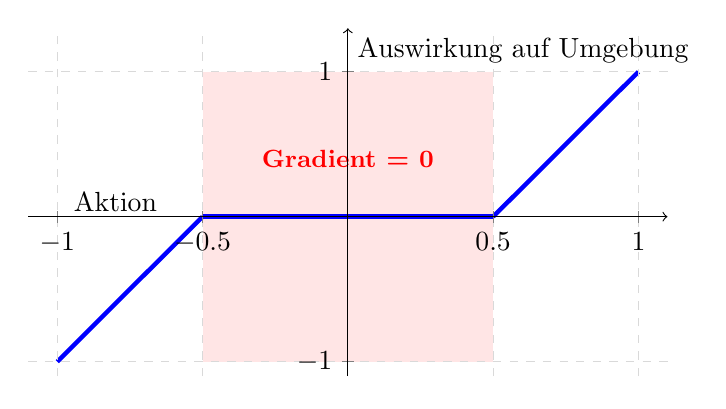
\begin{tikzpicture}
        \begin{axis}[
            width=0.8\textwidth,
            height=6cm,
            % xlabel is placed manually below using a node so it can be positioned
            % at a data coordinate (axis cs) in the negative region.
            ylabel={Auswirkung auf Umgebung},
            xmin=-1.1, xmax=1.1,
            ymin=-1.1, ymax=1.3,
            axis lines=middle,
            grid=major,
            grid style={dashed, gray!30},
            legend pos=north west,
            legend style={draw=none},
            xtick={-1, -0.5, 0, 0.5, 1},
            ytick={-1, 0, 1},
            % Improve axis line appearance
            axis line style={->},
            area style,
        ]
        
        % Deadzone shading
        \fill[red!10] (axis cs:-0.5,-1.0) rectangle (axis cs:0.5,1.0);
        
        % The function
        % Linear outside [-0.5, 0.5], zero inside
        \addplot[blue, ultra thick, domain=-1:-0.5] {2 * (x + 0.5)};
        \addplot[blue, ultra thick, domain=-0.5:0.5] {0};
        \addplot[blue, ultra thick, domain=0.5:1] {2 * (x - 0.5)};
        
        % Annotations
        \node[red, align=center, font=\small\bfseries] at (axis cs:0, 0.4) {Gradient = 0};

        % Manuelles xlabel an einer Datenkoordinate im negativen Bereich
        \node[align=center] at (axis cs:-0.8,0.1) {Aktion};

        \end{axis}
    \end{tikzpicture}
    \caption{Visualisierung des Deadzone-Problems: Die X-Achse repräsentiert die gewählte Aktion, die Y-Achse die resultierende Seitenschubdüsenleistung in der LunarLander-Umgebung.}
    \label{fig:deadzone_plot}
\end{figure}
\vspace{\baselineskip}

Die verwendeten Hyperparameter sind in Anhang \ref{lst:lunar_lander_hyperparams} dokumentiert. Der verwendete Environment Wrapper, der künstlich eine Abhängigkeit zwischen einer diskreten Aktivierungs-Aktion und der eigentlichen diskreten Steuerungsaktion erzeugt, ist in Listing \ref{lst:lunar_lander_wrapper} dargestellt. Dies ermöglicht den Vergleich der Lernkurven unter kontrollierten Bedingungen.
\vspace{\baselineskip}

Die zugrunde liegenden Hypothesen lauten wie folgt:
\begin{enumerate}
    \item \label{hyp:baseline} \textbf{Baseline-Performance:} Der Standard-PPO-Algorithmus erreicht in der regulären Umgebung eine durchschnittliche finale Belohnung von mindestens 270 \cite{algo_score_reference}.
    \item \label{hyp:no_gating} \textbf{Architektur-Robustheit:} Der PPO-Algorithmus ohne Gradient Gating zeigt in der modifizierten Umgebung keine signifikante Leistungsverschlechterung gegenüber dem Standard-PPO.
    \item \label{hyp:convergence} \textbf{Gating-Trade-off:} Der Einsatz von Gradient Gating führt initial zu einer verlangsamten Konvergenz (niedriger \emph{Mean Eval Mean}), resultiert jedoch in einer überlegenen finalen Policy (höherer \emph{Last Eval Mean}).
    \item \label{hyp:stability} \textbf{Stabilität:} Gradient Gating reduziert die Varianz zwischen den Trainingsläufen und erhöht die Lernstabilität signifikant.
    \item \label{hyp:Interferenzen} \textbf{Vermeidung negativer Interferenzen:} Die angepasste Netzarchitektur mit separaten Verarbeitungspfaden für diskrete und kontinuierliche Aktionen in Kombination mit Gradient Gating führt zu einer weiteren Leistungssteigerung gegenüber der Standard-Gradient-Gating-Variante, besonders in Scenarien mit eine hochen Anteil non -Noop Aktionen.
    \item \label{hyp:Netzarchitektur} \textbf{Netzarchitektur:} Die angepassten Netzarchitekturen sollten in diesm Scenario keine signifikante Leistungssteigerung gegenüber der Standard-Gradient-Gating-Variante zeigen, da alle Aktionen etwa gleich häufig auftreten und die Interferenz zwischen den Aktionszweigen gering sein sollten. 
\end{enumerate}

\subsubsection*{Durchführung}

Um die Effektivität des Gradient-Gating-Mechanismus und den Einfluss der Netzwerkarchitektur zu testen, werden die Experimente in zwei übergeordnete Testreihen gegliedert:

\begin{enumerate}
    \item \textbf{Testreihe 1: Validierung der Wirksamkeit des Gradient Gating} \\
    In dieser Phase wird geprüft, ob der Gating-Mechanismus gegenüber den Standard-Verfahren einen Vorteil bietet.
    \begin{itemize}
        \item \textbf{Standard PPO:} Der unveränderte Basis-Algorithmus in der Standard-Umgebung.
        \item \textbf{PPO mit Wrapper:} Der Standard-Algorithmus in der mittels Wrapper modifizierten Umgebung. Diese simuliert den gemischten Aktionsraum und dient als Baseline, um sicherzustellen, dass allein die Umgebungskapselung keine Leistungsänderung bewirkt.
        \item \textbf{PPO mit Gating:} Der Standard-Algorithmus in der modifizierten Umgebung, erweitert um den in Kapitel \ref{ch:ppo_bedingt} beschriebenen Gradient-Gating-Mechanismus.
    \end{itemize}

    \item \textbf{Testreihe 2: Analyse verschiedener Netzarchitekturen unter Gradient Gating} \\
    In dieser Phase werden verschiedene Netzwerk-Topologien evaluiert, die alle den Gating-Mechanismus nutzen.
    \begin{itemize}
        \item \textbf{PPO (Fully Shared):} Diese Variante nutzt dieselbe vollständig geteilte Architektur wie \textit{PPO mit Gating}, realisiert diese jedoch technisch über eine \textit{Aktionsnetzwerk-basierte Implementierung}. Dabei wird das vorgeschaltete Policy-Netzwerk leer initialisiert (\texttt{[]}) und die gesamte Topologie direkt im Aktionsnetzwerk abgebildet. Da die spezialisierten Split-Architekturen ebenfalls auf dieser Methode beruhen, dient diese Variante als interne Validierung, um methodische Abweichungen zur nativen Implementierung zu isolieren.
        \item \textbf{PPO (Split Net):} Das Netzwerk wird ab der Eingabeschicht in separate Äste für die unterschiedlichen Aktionen aufgeteilt. Um die Parametereffizienz vergleichbar zur Basis-Architektur zu halten, wird die Anzahl der Neuronen pro Ast reduziert. Die Dimensionierung erfolgt dabei gemäß der in Kapitel \ref{ch:ppo_bedingt} hergeleiteten Approximation (siehe Gleichung \ref{eq:complexity_approx}).
        \item \textbf{PPO (Split Net Full):} Eine Variante mit vollständig getrennten Netzwerken, bei der jeder Ast die volle Breite des ursprünglichen Netzwerks behält. Da jeder Pfad auch die Feature-Extraktion vollständig eigenständig erlernen muss, wird auf eine Reduktion der Parameter verzichtet.
        \item \textbf{PPO (Shared \& Split):} Ein hybrider Ansatz, der einen gemeinsamen Layer für die grundlegende Feature-Extraktion verwendet, gefolgt von getrennten Köpfen (Heads) für die Aktionen. Auch hier wird die Neuronenanzahl der getrennten Layer anhand der Formel (Gleichung \ref{eq:complexity_approx}) reduziert.
    \end{itemize}
\end{enumerate}

Jede Konfiguration wird mit den selben Hyperparamertern und den gleichen 15 Seeds trainiert, um die Vergleichbarkeit der Ergebnisse zu gewährleisten. Beim Bootstrap wurden 5000 Stichproben gezogen. Die Trainingsdauer beträgt jeweils 3 Million Zeitschritte.


\subsubsection*{Ergebnisse}

\begin{table}[htbp]
    \centering
    \caption{Vergleich der Trainingsergebnisse (IQM mit 95\%-Konfidenzintervall)}
    \label{tab:evaluation_results}
    \resizebox{\textwidth}{!}{%
    \begin{tabular}{cl|ccc|ccc}
        \toprule
        & & \multicolumn{3}{c}{\textbf{Last Eval}} & \multicolumn{3}{c}{\textbf{Mean Eval}} \\ 
        \multicolumn{2}{l|}{\textbf{Konfiguration}} & \textbf{Low} & \textbf{IQM} & \textbf{High} & \textbf{Low} & \textbf{IQM} & \textbf{High} \\
        \midrule
        \multirow{7}{*}{\rotatebox{90}{\textbf{Absolute Werte}}}
        & Standard PPO & 270.05 & 275.04 & 278.56 & 238.79 & 241.95 & 245.02 \\
        & PPO (with Wrapper) & 256.65 & 266.76 & 275.05 & 236.47 & 239.76 & 244.11 \\
        & PPO (Gating) & 284.20 & 287.41 & 289.28 & 167.43 & 188.50 & 205.07 \\
        & PPO (Fully Shared) & 278.64 & 285.12 & 286.67 & 179.59 & 194.76 & 203.68 \\
        & PPO (Split Net) & 284.45 & 286.09 & 287.09 & 179.32 & 193.35 & 204.17 \\
        & PPO (Split Net Full) & 277.56 & 283.11 & 285.47 & 180.10 & 188.88 & 196.58 \\
        & PPO (Shared \& Split) & 281.94 & 284.99 & 286.80 & 177.24 & 196.29 & 207.38 \\
        \midrule
        \multirow{6}{*}{\rotatebox{90}{\shortstack{\textbf{Pairdifferenz}\\ \scriptsize (Modell - Standard)}}} 
        & Wrapper & -18.59 & -8.19 & 1.75 & -7.03 & -2.22 & 3.96 \\
        & Gating & 6.74 & 12.28 & 18.17 & -73.79 & -53.60 & -36.27 \\
        & Fully Shared & 1.80 & 10.05 & 16.05 & -63.36 & -47.12 & -37.30 \\
        & Split Net & 7.12 & 11.03 & 16.19 & -62.47 & -48.63 & -36.57 \\
        & Split Net Full & 0.91 & 8.11 & 13.58 & -62.88 & -53.33 & -44.49 \\
        & Shared \& Split & 4.81 & 9.85 & 15.98 & -66.72 & -45.79 & -33.78 \\
        \bottomrule
    \end{tabular}%
    }
\end{table}

Die in Tabelle \ref{tab:evaluation_results} quantifizierten Daten belegen die Validität des Versuchsaufbaus und ermöglichen eine differenzierte Bewertung der beiden Testreihen.

\subsubsection*{Grundlegende Validierung}
Die Ergebnisse bestätigen, dass der experimentelle Rahmen solide ist. Der Standard-PPO erreicht mit einem IQM von 275.04 den geforderten Referenzwert (Bestätigung Hypothese \ref{hyp:baseline}). Zudem zeigt das Konfidenzintervall der Wrapper-Variante $[-18.59, 1.75]$ (Differenz zu Standard-PPO), dass die Kapselung der Umgebung selbst keinen signifikanten Einfluss auf die Leistung hat (Bestätigung Hypothese \ref{hyp:no_gating}). Dies isoliert den Gating-Mechanismus als die alleinige Ursache für die im Folgenden diskutierten Effekte.

\subsubsection*{Testreihe 1: Wirksamkeit des Gradient Gating}
Der Vergleich zwischen Standard-PPO und PPO mit Gating offenbart den postulierten Trade-off (Hypothese \ref{hyp:convergence}):
Während der Gating-Ansatz über das gesamte Training hinweg eine niedrigere Durchschnittsleistung (\emph{Mean Eval Mean}) aufweist, was auf die initialen Lernkosten der hierarchischen Struktur zurückzuführen ist, zahlt sich diese Investition am Ende aus. Das positive Paird-Intervall für die finale Leistung (`Last Eval Mean`: $[6.74, 18.17]$) belegt, dass der Gating-Mechanismus zu einer signifikant leistungsfähigeren finalen Policy führt.
\begin{figure}[htbp]
    \centering
    \includegraphics[width=0.9\textwidth]{chapters/bilder/iqm_ci_LunarLanderContinuous-v3_last_eval_mean.png}
    \caption{Finale Trainingsleistung (Last Eval)}
    \label{fig:iqm_last_eval}
\end{figure}

Gleichzeitig bestätigt sich Hypothese \ref{hyp:stability} bezüglich der Stabilität. Wie in Abbildung \ref{fig:iqm_last_eval} ersichtlich, konvergiert der Gating-Ansatz robuster (schmaleres Konfidenzintervall von 5.08) als die Standard-Variante (8.51). Die Performance Profiles (Abbildung \ref{fig:perf_profile_last_eval}) unterstreichen dies durch die stochastische Dominanz der Gating-Kurve, die insbesondere im hohen Leistungsbereich stabil bleibt.

\begin{figure}[htbp]
    \centering
    \includegraphics[width=0.9\textwidth]{chapters/bilder/iqm_ci_LunarLanderContinuous-v3_mean_eval_mean.png}
    \caption{Durchschnittliche Trainingsleistung (Mean Eval)}
    \label{fig:iqm_mean_eval}
\end{figure}

\subsubsection*{Testreihe 2: Performance der Architekturen}
Bei der Analyse der Netzwerkarchitekturen ist zunächst eine methodische Besonderheit zu beachten. Um die verschiedenen Topologien flexibel zu realisieren, wurde für diese Testreihe eine \textit{Aktionsnetzwerk-basierte Implementierung} gewählt, bei der die Netzstruktur technisch in das Aktionsnetzwerk verlagert wurde. Ein Vergleich der \textit{PPO (Fully Shared)} Variante (welche diese Methode nutzt) mit der nativen \textit{PPO mit Gating} Implementierung zeigt einen leichten Leistungsabfall (IQM 285.12 vs. 287.41). Dies deutet auf minimale Ineffizienzen durch diese technische Realisierung hin.
Aus diesem Grund werden die Architekturen im Folgenden relativ zueinander bewertet, wobei \textit{PPO (Fully Shared)} als interne Baseline dient.
\vspace{\baselineskip}

In diesem direkten Vergleich schneidet die \textit{PPO (Split Net)} Architektur am besten ab (IQM 286.09). Sie übertrifft die Fully\hyp{}Shared\hyp{}Baseline, wenngleich die Überlappung der Konfidenzintervalle keine statistische Signifikanz ausweist. Dennoch stützt dieses Ergebnis Hypothese \ref{hyp:Netzarchitektur}: Die Trennung der Pfade (bei gleichzeitiger Reduktion der Neuronenanzahl zur Wahrung der Parameter\hyp{}Effizienz) scheint vorteilhaft zu sein, da sie spezialisierte Repräsentationen ohne negativen Einfluss erlaubt.
Die komplexeren Varianten (\textit{Split Net Full}, \textit{Shared \& Split}) zeigen hingegen keine Vorteile. Dies lässt vermuten, dass die erhöhte Parameteranzahl in dieser vergleichsweise einfachen Umgebung keinen Mehrwert bietet und tendenziell eher zu Overfitting führt.
\vspace{\baselineskip}

Zusammenfassend lässt sich festhalten, dass der Gating\hyp{}Mechanismus der entscheidende Faktor für den Leistungsgewinn ist.
Die Wahl der Netzarchitektur spielt in diesem Szenario eine untergeordnete Rolle, wobei die effiziente \textit{Split Net}-Struktur das vielversprechendste Potenzial für komplexere Aufgaben (wie die Flugverkehrskontrolle) andeutet.

\begin{figure}[htbp]
    \centering
    \includegraphics[width=0.8\textwidth]{chapters/bilder/perf_profile_LunarLanderContinuous-v3_last_eval_mean.png}
    \caption{Performance Profile der finalen Leistung}
    \label{fig:perf_profile_last_eval}
\end{figure}

\subsection{Versuch 2: Validierung in der Flugverkehrsumgebung}

Nachdem die grundlegende Funktionalität des Gradient\hyp{}Gating\hyp{}Mechanismus am Beispiel des Lunar Landers validiert wurde, folgt nun die Untersuchung in der eigentlichen Zieldomäne: der Flugverkehrskontrolle. Diese Umgebung stellt deutlich höhere Anforderungen an den Agenten, da sowohl die Dynamik komplexer ist als auch die Sicherheitsanforderungen strikter sind.

\begin{figure}[h]
    \centering
    \includegraphics[width=0.8\textwidth]{chapters/bilder/atc_env.png}
    \caption{Die Simulationsumgebung BlueSky}
    \label{fig:atc_env}
\end{figure}

Ein wesentlicher Unterschied zum vorangegangenen Versuch liegt in der Spärlichkeit der Konflikte (Sparse Rewards). Da tatsächliche Konfliktsituationen selten auftreten, ist ein rein reaktives Lernen ineffizient. Um dem Agenten dennoch ein stetiges und informatives Lernsignal zu bieten, wurden Belohnungsfunktion und Beobachtungsraum signifikant erweitert. Die Einbeziehung prädiktiver Faktoren – wie potenzieller zukünftiger Konfliktpunkte – sowie komplexer Metriken zu benachbarten Flugzeugen und der Routeneffizienz erhöht die Dimensionalität des Problems drastisch. Dies führt zu einer weitaus anspruchsvolleren Systemdynamik, die im Vergleich zur LunarLander-Umgebung deutlich höhere Anforderungen an die Lernstabilität des Algorithmus stellt.
\vspace{\baselineskip}

Die Hypothesen für diesen Versuch lauten:
\begin{enumerate}
    \item \label{hyp:atc_stability} \textbf{Lernstabilität in komplexer Umgebung:} Der Gradient\hyp{}Gating\hyp{}Mechanismus ermöglicht auch in der hochdimensionalen ATC-Umgebung ein stabiles Training und verhindert den Kollaps der Policy.
    \item \label{hyp:atc_performance} \textbf{Performance-Gewinn:} Der Agent mit Gating erreicht eine höhere durchschnittliche Belohnung als der Standard-Agent, da er feinfühligere Steuerbefehle erlernen kann, ohne durch das Rauschen irrelevanter Aktionen gestört zu werden.
    \item \label{hyp:atc_architecture} \textbf{Architektureffizienz:} Analog zum ersten Versuch wird erwartet, dass spezialisierte Architekturen (wie Split Net) die Lernleistung weiter verbessern können.
\end{enumerate}

\subsubsection*{Durchführung}

Im Gegensatz zum vorherigen Versuch wird die Evaluation in der Flugverkehrsumgebung aufgrund der enormen Rechenkomplexität auf eine einzelne, konsolidierte Testreihe beschränkt. Zwei Faktoren sind hierfür ausschlaggebend: Erstens ist die Interaktion mit dem externen Simulator (BlueSky) um ein Vielfaches zeitintensiver als mit einfachen Gym-Umgebungen. Zweitens erfordert die Lösung des ATC-Problems ein breiteres neuronales Netz und eine deutlich längere Trainingsdauer, um eine stabile Policy zu erlernen.

Daher werden die folgenden vier Konfigurationen in einem gemeinsamen Szenario evaluiert:
\begin{itemize}
    \item \textbf{PPO:} Der Standard-Algorithmus als Baseline.
    \item \textbf{Masked PPO:} Der PPO-Algorithmus erweitert um den Gradient-Gating-Mechanismus.
    \item \textbf{Masked split\_net PPO:} Die Variante mit getrennten Netzpfaden für diskrete und kontinuierliche Aktionen.
    \item \textbf{Masked shared \& split\_net PPO:} Die hybride Architektur mit geteiltem Feature-Extractor.
\end{itemize}
Dies gewährleistet die direkte Vergleichbarkeit unter identischen Bedingungen bei vertretbarem Ressourcenaufwand.

Die Trainingsdauer wird auf [6] Millionen Zeitschritte festgelegt. Es werden 7 Seeds verwendet.

\subsubsection*{Ergebnisse}

\begin{table}[htbp]
    \centering
    \caption{Vergleich der Trainingsergebnisse in der Flugverkehrsumgebung (IQM mit 95\%-Konfidenzintervall)}
    \label{tab:atc_evaluation_results}
    \resizebox{\textwidth}{!}{%
    \begin{tabular}{cl|ccc|ccc}
        \toprule
        & & \multicolumn{3}{c}{\textbf{Last Eval}} & \multicolumn{3}{c}{\textbf{Mean Eval}} \\ 
        \multicolumn{2}{l|}{\textbf{Konfiguration}} & \textbf{Low} & \textbf{IQM} & \textbf{High} & \textbf{Low} & \textbf{IQM} & \textbf{High} \\
        \midrule
        \multirow{4}{*}{\rotatebox{90}{\textbf{Absolute Werte}}}
        & PPO & 0.00 & 0.00 & 0.00 & 0.00 & 0.00 & 0.00 \\
        & Masked PPO & 0.00 & 0.00 & 0.00 & 0.00 & 0.00 & 0.00 \\
        & Masked split\_net PPO & 0.00 & 0.00 & 0.00 & 0.00 & 0.00 & 0.00 \\
        & Masked shared \& split\_net PPO & 0.00 & 0.00 & 0.00 & 0.00 & 0.00 & 0.00 \\
        \midrule
        \multirow{3}{*}{\rotatebox{90}{\shortstack{\textbf{Pairdifferenz}\\ \scriptsize (Modell - PPO)}}} 
        & Masked PPO & 0.00 & 0.00 & 0.00 & 0.00 & 0.00 & 0.00 \\
        & Masked split\_net PPO & 0.00 & 0.00 & 0.00 & 0.00 & 0.00 & 0.00 \\
        & Masked shared \& split\_net PPO & 0.00 & 0.00 & 0.00 & 0.00 & 0.00 & 0.00 \\
        \bottomrule
    \end{tabular}%
    }
\end{table}

[Hier Text einfügen: Analyse der Tabelle, Bestätigung oder Widerlegung der Hypothesen.]

\begin{figure}[htbp]
    \centering
    % TODO: Plot einfügen
    %\includegraphics[width=0.9\textwidth]{chapters/bilder/iqm_ci_atc_last_eval.png}
    \caption{Finale Trainingsleistung (Last Eval) - Flugverkehr}
    \label{fig:iqm_atc_last_eval}
\end{figure}

[Hier Text einfügen: Diskussion der Performance Profiles oder Lernkurven.]




\section{Evaluation des Aktionsraum-Designs}
\subsection{Vergleich: Gemischter vs. Diskreter Aktionsraum}
In diesem zentralen Experiment werden die Leistungsunterschiede zwischen dem neu konzipierten Agenten mit gemischtem Aktionsraum und einem Referenz-Agenten untersuchten. Der Referenz-Agent nutzt einen klassischen, rein diskreten Aktionsraum (feste Menge an Kursänderungen), wie er in vielen bisherigen Arbeiten verwendet wird.
Besonderes Augenmerk liegt hierbei nicht nur auf der reinen Konfliktfreiheit (Success Rate), sondern auf der Qualität der generierten Trajektorien: Wie oft greift der Agent ein? Wie effizient sind die Routen?

\section{Fazit der Ergebnisse}



